\cotefile{136}

\scanpage{33}

donc $C_{l,i+j}$ et $C_{l+j,i}$ $\not\equiv 0\ (p)$. C'est le contenu du

\uline{Lemme 2} Soient $i,j\geq 0$. Alors il existe $l\geq 0$ tel que \deleted{\unsure{$C_{i+j,l}$}} $C_{i+j,l}$ et $C_{i,j+l}$ soient $\not\equiv 0\ (p)$.

\deleted{\uline{Dém.} Considérons \unsure{les|des} développements $p$-adiques de $i$ et $j$

\[
\begin{aligned}
i&=i_0+i_1p+\cdots+i_rp^r\\
j&=j_0+j_1p+\cdots+j_rp^r
\end{aligned}
\]

alors le développement $p$-adique de \inserted{$\sigma=$}$i+j$ est \inserted{$\deleted{\unsure{i+}}j=\sigma=\sigma_0+\sigma_1p+\cdots+\sigma_{r+1}p^{r+1}$} donné par le procédé \unsure{vraiment|usuel} bien connu, où on détermine par récurrence des couples d'entiers $\sigma_\alpha$, \deleted{\unsure{$\rho_\alpha$}} $(0\leq\alpha\leq r+1)$ \inserted{et $\rho_\alpha$ $(-1\leq\alpha\leq r)$}

-- les $\rho_\alpha$ sont les ``retenues'', égales soit à $0$ ou $1$ -- en posant \deleted{\illegible{1}} \textcircled{a} $\rho_{-1}=0$, puis par récurrence par

\[
\underset{\downarrow}{\text{\textcircled{$0\leq\alpha\leq r\deleted{\unsure{+}}$}}}
\quad\text{\textcircled{b}}\quad i_\alpha+j_\alpha+\rho_{\alpha-1}=\sigma_\alpha+p\rho_\alpha
\qquad 0\leq\sigma_\alpha,\unsure{p|\rho}_\alpha\leq p-1
\]

celà détermine $\sigma_\alpha$ et $\rho_\alpha$

\[
\text{enfin}\quad \text{\textcircled{c}}\qquad \sigma_{\alpha+1}=\rho_{\unsure{r|\alpha}}
\]

Posons

\[
\begin{aligned}
l_\alpha&=(p-1)-\sigma_\alpha\qquad 0\leq\alpha\leq r+1\\
l&=\sum_{0}^{r+1}l_\alpha p^\alpha
\end{aligned}
\]

\[
\text{d'où}\qquad \sigma+l=\sum_0^{r+1}(p-1)p^\alpha=p^{r+2}-1\qquad \text{i.e.}\quad l=p^{r+2}-1-\sigma
\]

On a alors, grâce à (b)

\[
\text{\textcircled{$a'$}}\qquad \rho_{-1}=0
\]

\[
\text{\textcircled{$b'$}}\quad\text{Si }0\leq\alpha\leq r,\quad
(i_\alpha+j_\alpha+l_\alpha)+\rho_{\alpha-1}=(p-1)+p\rho_\alpha
\quad\left(\begin{gathered}\text{où }\unsure{\alpha-1|\rho_{\alpha-1}|\sigma_\alpha}\\
\text{et }\rho_\alpha\text{ sont}\\0\leq\ \ \leq p-1\end{gathered}\right)
\]

\[
\text{\textcircled{$b'$ bis}}\quad\deleted{\unsure{i_{r+1}}}\quad
\underset{\substack{\shortparallel\\0}}{i_{r+1}}+\underset{\substack{\shortparallel\\0}}{j_{r+1}}+l_{r+1}+\rho_r=(p-1)+p\mathbin{.}0
\]

\deleted{\textcircled{$c'$}} \deleted{\unsure{$i+j$}} Ce qui montre que \deleted{\unsure{lorsque}} l'addition des}

% archive sheet number: 32
\scanpage{34}

\deleted{entiers $i,j,l$, donnés par leurs développements $p$-adiques}

Soit $r\geq 0$ tel que $p^r>i+j$, soit \deleted{\unsure{$l=$}}

\[
l=p^r-1-(i+j)
\]

\deleted{Je dis que} de sorte que l'on a

\[
\underset{\substack{\rotatebox{25}{$=$}\\\inserted{(i+j)+l=i+(j+l)}}}{i+j+l}=p^r-1=\sum_{\alpha=0}^{r-1}(p-1)p^\alpha
\]

On sait alors, par le critère habituel, que l'on a $C_{i+j,l}\not\equiv 0\ (p)$, et pour la $=$ raison on a $C_{\unsure{j|i},j+l}\not\equiv 0\ (p)$

cqfd

\uline{NB} Le lemme commun qui a servi dans les lemmes 1 et 2 est le suivant :

Si $\mu,\nu\geq 0$ sont tels que

\[
\mu+\nu=p^r-1\qquad (r\geq 0\ \text{convenable})
\]

\[
\text{alors}\qquad C_{\mu,\nu}\not\equiv 0\ (p)
\]

\deleted{(plus précisément, $C_{\mu,\nu}$}

% archive sheet number: 33
\scanpage{35}

\[
\boxed{\unsure{V|\nu|v}_p(n!)=\frac{n-\mathrm{chif}_p\,n}{p-1}}
\]

\[
\begin{aligned}
\deleted{V_p(n!)}\quad V_p\left(\frac{p^n}{n!}\right)&=n-\frac{n-\mathrm{chif}_p\,n}{p-1}\\
&=\frac{\mathrm{chiff}_p(n)+n(p-2)}{p-1}
\end{aligned}
\]

\[
\begin{aligned}
n&=\sum_{\alpha\geq 0}n_\alpha p^\alpha\\
\mathrm{chif}_p\,n&=\sum n_\alpha
\end{aligned}
\]

\[
\begin{aligned}
n-\mathrm{chif}_p\,n&=\sum n_\alpha(p^\alpha\deleted{\unsure{-}}-1)\\
\frac{n-\mathrm{chif}_p\,\unsure{n)|n}}{p-1}&=\sum_\alpha n_\alpha(1+\cdots+p^{\alpha-1})
\end{aligned}
\]

\[
V_p((n+1)!)=
\]

\[
\begin{aligned}
V_p\left(\frac{p^{r+1}!}{(p^r!)^p\,p!}\right)
&=\underset{\frac{p^{r+1}-1}{p-1}}{\underline{V_p(p^{r+1}!)}}-p\,\underset{\frac{p^r-1}{p-1}}{\underline{V_p(p^r!)}}-\underset{1}{\underline{V_p(p!)}}\\
&=0
\end{aligned}
\]

% archive sheet number: 34
\scanpage{36}

aux homomorphismes

\[
T\longrightarrow A^{\handwritten{\natural}}\longrightarrow A\ ,
\]

nous montre alors aussitôt que $\underline{F}(A^{\handwritten{\natural}})$ et $\underline{F}(T)$ s'identifient respectivement à

\[
\tag*{(13.4.10)}
\underline{F}(A^{\handwritten{\natural}})\simeq\underline{F}^{f}\overset{\mathrm{dfn}}{=}\underline{F}\cap\mathcal{E}^{f}\ ,\quad \underline{F}(T)=\underline{F}^{t}=\underline{F}\cap\mathcal{E}^{t}=0\ ,
\]

le $=0$ provenant du fait immédiat que pour un tore $T$, on a $\underline{F}(T)=0$, la suite exacte du type (13.4.3) devenant ici $0\to0\to\mathcal{E}(T)\to\underline{\mathrm{Lie}}(T)\to0$.

On voit donc en même temps que l'homomorphisme composé

\[
\mathcal{E}^{t}\longrightarrow\mathcal{E}\longrightarrow\underline{E}
\]

induit un isomorphisme

\handwritten{\mspage{495}}

\mspage{495}

% archive sheet number: 35
\scanpage{37}

\[
\begin{aligned}
\mathrm{Hom}^{d}(M^{*},\varphi_N N^{*})&=\mathrm{Hom}(M^{*}[-d],\varphi_N N^{*})\\
&\simeq\mathrm{Hom}(\tau_N(M^{*}[-d]),N^{*})\\
&\simeq\mathrm{Hom}((\tau_{N-d}M^{*})[-d],N^{*})\\
&\simeq\mathrm{Hom}^{d}(\tau_{N-d}M^{*},N^{*})
\end{aligned}
\]

\margin{$N^{*}\in\mathrm{Ob}\,\mathcal{M}_N$}

\[
\boxed{\mathrm{Hom}^{d}(M^{*},\varphi_N N^{*})\simeq\mathrm{Hom}^{d}(\tau_{N-d}M^{*},N^{*})}
\]

\uline{Supposons} $M^{*}\in\mathcal{M}^{*}_{\deleted{\unsure{d}}-d}$ $[\text{i.e. } M^{j}=0\text{ si }j<-d]$,

\[
\begin{aligned}
\mathcal{N}^{*}&=\tau_N N\otimes_k S_k\deleted{\unsure{=}}=\tau_N\mathcal{N}_{S_k}\quad (N\text{ un }k\text{-module})\\
&\quad N\geq 0
\end{aligned}
\]

\[
\begin{aligned}
\text{Alors }\quad\mathrm{Hom}^{d}(M^{*},\varphi_N\tau_N\mathcal{N}^{*}_{S_k})
&=\mathrm{Hom}^{d}(M^{*},\underbrace{\varphi_{\unsure{\infty N|N}}\tau_N\mathcal{N}^{\unsure{\alpha|*}}_{S_k}}_{=\tau_N\varphi_N\tau_N\mathcal{N}^{\unsure{*|s}}_{S_k}})=\mathrm{Hom}^{d}(M^{*},\tau_N\\
&=\unsure{\mathrm{H}}
\end{aligned}
\]

\figure{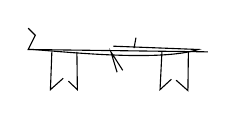
\begin{tikzpicture}[x=6mm,y=6mm]
\draw (0,.5)--(.15,.35)--(0,.05)--(3.8,0);
\draw (.1,.05) .. controls (1,-.02) and (2.8,-.2) .. (3.6,.05) -- (1.8,.12);
\draw (.5,0)--(.47,-.8)--(.74,-.56) (1.03,0)--(1.04,-.8)--(.85,-.62)
 (1.88,-.43)--(1.75,0)--(2,-.39) (2.28,.3)--(2.24,.08)
 (2.83,0)--(2.79,-.8)--(3.03,-.58) (3.39,0)--(3.38,-.82)--(3.13,-.6);
\end{tikzpicture}}

% The following cancelled block is written upside down.

\deleted{\[
\boxed{G,\quad g_1,\quad\ \ ,g_r}\quad
\begin{gathered}\longrightarrow\\[-2pt]\twoheadrightarrow\end{gathered}
\]

Diagramme de Cayley

\diagram{\begin{tikzcd}[ampersand replacement=\&,row sep=5mm,column sep=7mm,
execute at end picture={
\begin{scope}[shift={(\tikzcdmatrixname-2-2.center)},x=1cm,y=1cm]
\draw (0,0) .. controls (0,1.9) and (1.85,2.8) .. (3.05,1.9) .. controls (4,1.2) and (1.65,.65) .. (0,0);
\draw[->] (0,0)--(.04,.46);\draw (.04,.46)--(.09,1);
\draw (0,0)--(1.42,.98);\draw[->>] (0,0)--(.38,.22);
\draw[->>] (.09,1)--(.63,1.2);\draw[->>] (0,0)--(.34,-.36);
\draw (-.22,-.42)--(0,0);
\fill (.09,1) circle(1.8pt) (1.42,.98) circle(1.5pt) (0,0) circle(1.8pt);
\node[below] at (.05,0) {$x$};\node[right] at (1.36,.75) {$xg_i$};
\fill (-1.45,.03) circle(1.2pt) (-1.38,-.27) circle(1.2pt) (1.55,0) circle(1pt) (3,0) circle(1.2pt) (4.65,-.13) circle(1pt);
\draw (4.68,-.34) .. controls (6.1,-.1) and (7.8,-.2) .. (7.12,1.23);
\node[below] at (4.71,-.33) {$\unsure{y|g}$};
\draw[thin] (-.67,1.98)--(1.76,-1.63) (3.1,2.25)--(5.85,-1.78);
\end{scope}}]
\vphantom{x}\&\vphantom{x}\\
\vphantom{x}\&\vphantom{x}
\end{tikzcd}}

Mot en les $g_i$ $+$ origine

$g,\ g_i$}

% archive sheet number: 36
\scanpage{38}

\mspage{- 180 -}\hfill IX

\uline{En d'autres termes}, \uline{la filtration de} $\mathcal{E}^{t}$ \uline{induite par la filtration de Hodge} (\uline{avec les conventions de degrés} (13.4.6)) \uline{est concentrée en degré} $-1$, \uline{celle de} $\mathcal{E}/\mathcal{E}^{f}$ \uline{induite par la filtration de Hodge est concentrée en degré} $0$.

c) \uline{Considérons la filtration de}

\[
\mathcal{E}^{\mathrm{ab}}\overset{\mathrm{dfn}}{=}\mathcal{E}^{f}/\mathcal{E}^{t}\simeq
(\underline{R}^{\mathrm{ab}})\otimes_{\mathbb{Z}}\underline{O}_S
\quad,\quad \text{où }\underline{R}^{\mathrm{ab}}=\underline{R}^{f}/\underline{R}^{t}\quad\text{(cf. a))}\quad,
\]

\uline{induite par la filtration de Hodge de} $\mathcal{E}$,\uline{donc} \uline{définie par le sous-Module} $\underline{F}^{\mathrm{ab}}$ \uline{de} $\mathcal{E}^{\mathrm{ab}}$ \uline{image de}

\[
\underline{F}^{f}\overset{\mathrm{dfn}}{=}\underline{F}\cap\mathcal{E}^{f}\longrightarrow\mathcal{E}^{\mathrm{ab}}\quad ,
\]

(\uline{la flèche étant un monomorphisme grâce à la première relation} (*)).

\uline{Alors le couple} $(\underline{\mathbb{R}}^{\mathrm{ab}},\underline{F}^{\mathrm{ab}}\subset\underline{\mathbb{R}}^{\mathrm{ab}}\otimes_{\mathbb{Z}}\underline{O}_S=\mathcal{E}^{\mathrm{ab}})$ \uline{est isomorphe au couple} $(\underline{R}(B),\underline{F}(B))$ \uline{associé à un} groupe abéloide \uline{sur} $S$, \uline{comme expliqué après} (13.4.4) (\uline{où donc} $B\simeq\mathcal{E}^{\mathrm{ab}}/(F^{\mathrm{ab}}+R^{\mathrm{ab}})$, \uline{les symboles non soulignés désignant les groupes analytiques sur} $S$ \uline{correspondants}).

\uline{Remarque} 13.4.18. Dans la terminologie de DELIGNE [4], la conclusion de la proposition précédente, lorsqu'on se restreint au-dessus d'un ouvert $U$ de $S$ sur lequel $R$ est localement constant, exprime que $\unsure{\mathbb{R}|R}$, muni des deux filtrations (13.4.17.1) de $\mathcal{E}=\underline{\mathbb{R}}\otimes_{\mathbb{Z}}\underline{O}_S$, est une "famille analytique de structures de Hodge mixtes sur $U$ ". La situation qu'on vient d'expliciter a servie de modèle aux conjectures de DELIGNE sur la théorie de Néron en dimensions supérieures, énoncées dans [9, 9.8 à 9.13]. Il y a cependant un trait important de la théorie algébrique

\handwritten{\mspage{498}}

\mspage{498}

% archive sheet number: 37
\scanpage{39}

d'où

\[
\boxed{\mathrm{Hom}^{d}(M^{*},\deleted{\unsure{\varphi_N}}N\otimes_k S_k)\simeq\mathrm{Hom}^{d}(\tau_{N-d}M,\tau_N(N\otimes_k S_k)}
\]

\[
\text{Si }\left\{\begin{aligned}M^{*}&\in\mathcal{M}_{-d}\\ N&\geq0\end{aligned}\right.
\]

p. ex.

\[
\boxed{\begin{aligned}
\mathrm{Hom}^{d}(M\otimes_k S_k,N\otimes_k S_k)&\xrightarrow{\sim}\mathrm{Hom}^{d}(\tau_{N-d}M_{S_k},\tau_N N_{S_k}\\
\rotatebox{90}{$\simeq$}\qquad&\\[-3pt]
\mathrm{Hom}^{\deleted{\unsure{d}}}_k(M,N)&\qquad \text{\uuline{si $d\geq0$}},N\geq0
\end{aligned}}
\]

Hom. \unsure{hom|homogènes} de degré $d\in\mathbb{Z}$

\[
\tau_\alpha M_{S_k}\longrightarrow\tau_\beta N_{S_k}\qquad(\beta\geq\alpha)
\]

a) \deleted{$d\geq0$}. Supposons d'abord $\boxed{d\geq\beta-\alpha}$ i.e $\alpha+d\geq\beta$

On a \deleted{$\mathrm{Hom}^{i}(M$}-

\[
\begin{aligned}
\mathrm{Hom}^{d}(\tau_\alpha M_{S_k},\tau_\beta N_{S_k})&\overset{\sim}{\longleftrightarrow}\mathrm{Hom}^{d}(\tau_\alpha M_{S_k},\underbrace{\tau_{\alpha+i}\tau_\beta N_{S_k}}_{=\tau_{\alpha+d}N_{S_k}})\\
&\xleftarrow{\sim}\mathrm{Hom}^{d}(M_{S_k},N_{S_k})\simeq\mathrm{Hom}_k(M,N)
\end{aligned}
\]

(Si $u:M\mathord{-} N$, il lui correspond l'hom

\[
\underset{j\geq\alpha}{mT^{(j)}}\longmapsto u(m)T^{(d)}T^{(j)}=C_{d,j}\,u(m)T^{(d+j)}\qquad\bigg)
\]

b) Supposons $0\leq d<\beta-\alpha$ \inserted{\deleted{\unsure{d'où|i.e.}} $\beta\geq\beta-d\unsure{>|\geq}\alpha$}, on a alors

\deleted{\[
\begin{aligned}
\mathrm{Hom}^{d}(\tau_\alpha M_{S_k},\tau_\beta N_{S_k})&\underset{\unsure{\sim|\text{inj.}}}{\longrightarrow}\mathrm{Hom}^{d}(\tau_{\beta-d}M_{S_k},\tau_\beta N_{S_k})\\
&\hspace{40mm}\rotatebox{90}{$\simeq$}\\[-4pt]
&\hspace{36mm}\mathrm{Hom}_k(M,N)
\end{aligned}
\]}

% archive sheet number: 38
\scanpage{40}

\mspage{. 7 .}

$\circ$ \uline{Matériel commandé par Mme LATOUR}

Mme LATOUR a commandé par simple lettre, en prévision de l'attribution d'un contrat de recherche, un caisson climatique sur mesure et un enregistreur, fourni il y a deux ans par la SECASI, non réglé à ce jour.

Mme LATOUR n'était aucunement habilitée à passer cette commande. Le Conseil Scientifique pense que l'Université n'est nullement engagée par cette commande tout à fait irrégulière. Le Président fait remarquer que l'Université est obligée de payer car ce matériel, bien que toujours en caisse, a été reçu à l'U.S.T.L. depuis 2 ans, et que toutes les tentatives pour le faire reprendre par le fournisseur sont demeurées vaines.

Il propose de récupérer , sur une période de 5 ans, le montant de la commande, sur les points chercheurs qui concernent Mme LATOUR.

Le Conseil Scientifique donne son accord sur cette procédure.

.VIII. \uuline{EXAMEN DE LA PROPOSITION DE M. MORET}

( voir Page 4 du procès-verbal du Conseil Scientifique du 21 Mars 1975)

a) \uline{Modification des fiches chercheurs}

Après discussion,M. SIAU signale qu'une fiche est déjà établie pour chaque Maître Assistant en vue de l'avancement au choix. Si le Conseil Scientifique le désire, il peut avoir communication de ces fiches.

b) \uline{Répertoire des chercheurs qui ne publient pas depuis plusieurs années}

Ce travail sera confié à la Commission chargée d'étudier les rapports d'activité scientifique déjà parus (P.5 du procès verbal du 21 Mars dernier).

c) \uline{Publication nominative de toutes les heures supplémentaires}

Le Président R\unsure{O}UZAUD signale qu'il est très attentif au nombre d'heures supplémentaires attribuées à chaque enseignant de l'USTL, mais ne peut vérifier les heures supplémentaires assurées pour des organismes privés.

M. VIERNE souhaiterait qu'une information plus large sur les services assurés par les enseignants soit donnée.

Le Président ROUZAUD pense que le tableau des services pourrait être porté sur les tableaux d'affichage des commissions de spécialistes.

% archive sheet number: 39
\scanpage{41}

\[
\mathrm{Hom}^{d}(\tau_\alpha M_{S_k},\underset{\substack{\cap\\\tau_{\alpha+d}N_{S_k}}}{\underline{\tau_\beta N_{S_k}}})
\hookrightarrow\mathrm{Hom}^{d}(\tau_\alpha M_{S_k},\tau_{\alpha+d}N_{S_k})
\]

% The oblique leader starts at the left Hom in the preceding display.
\inserted{(sous-mod. des hom de degré $d$ de $\tau_\alpha M_{S_k}$ \unsure{ds|dans} $\tau_{\alpha+d}N_{S_k}$ qui veulent bien appliquer $\tau_\alpha M_{S_k}$ dans $\tau_\beta N_{S_k}\subset\tau_{\alpha+d}N_{S_k}$)}

\[
\overset{\rotatebox{90}{$\simeq$}}{\mathrm{Hom}_k(M,N)}
\]

Il faut donc prendre les $u:M\longrightarrow N$ tels que l'hom correspondant $\tau_\alpha M_{S_k}\mathord{-}\tau_{\alpha+d}N_{S_k}$

\[
mT^{(j)}\longmapsto C_{d,j}\,u(m)T^{(d+j)}
\]

\deleted{applique $M_S$} a son image dans $\tau_\beta N_{S_k}$, i.e. tels que

\[
\left\{\begin{aligned}
C_{d,\alpha}u&=0\\
C_{d,\alpha+1}u&=0\\
&\cdots\\
C_{d,\beta-d}u&=0
\end{aligned}\right.
\]

(ce qui s'écrit

\[
C_{d,j}\,u=0\quad\text{si}\quad\alpha\leq j<\underset{\deleted{\unsure{\beta-d+1}}}{\beta-d}\qquad\bigg)
\]

c) \uline{$d<0$}. Notons que

\[
N^{*}_{\deleted{\otimes}S_k}=\varphi_{0\beta}\tau_\beta N_{S_k}=\tau_0\underset{\substack{\cap\\\varphi_\beta N_{S_k}}}{\varphi_\beta\tau_\beta N_{S_k}}
\]

donc \inserted{si $M^{*}\in\mathrm{Ob}\,\mathcal{M}^{\unsure{*|\prime}}$}

\[
\begin{aligned}
\mathrm{Hom}^{d}(M^{*},N_{S_k})&\subset\mathrm{Hom}^{d}(M^{*},\varphi_\beta\tau_\beta N_{S_k})\\
&\hspace{9mm}\shortparallel\\
&\mathrm{Hom}(M^{\unsure{\prime|*}}[-d],\varphi_\beta N_{S_k})\\
&\hspace{9mm}\shortparallel\\
&\mathrm{Hom}(\tau_\beta M^{\prime}[-d],N_{S_k}
\end{aligned}
\]

% archive sheet number: 40
\scanpage{42}

\mspage{. \unsure{6|b} .}

Le Conseil Scientifique décide de répondre par la négative étant donné que la succession d'un laboratoire suppose l'acceptation de l'actif et du passif et que le reliquat 1973 laissé par Mle TUZET s'élevait à 18.956 F 23.

$\circ$ \uline{Demande de M. MATTAUER}

M. MATTAUER fait état d'un appareil de son laboratoire endommagé à la suite du branchement d'eau en 1973. En l'absence d'information plus complète, le Conseil Scientique surseoit à l'examen de cette demande.

Un rapport plus détaillé sera demandé à l'intéressé.

$\circ$ \uline{Demande de M.M. MATTAUER et LOUIS}

Demande de subvention pour couvrir les frais d'impression de la troisième réunion des Sciences de la Terre (23,24 et 25 avril 1975, à l'U.S.T.L.) qui s'élève à 9.313 F 96.

Cette subvention est accordée.

$\circ$ \uline{Demande de M. MORETTI}

19.000 F pour faire réparer un analyseur d'acides aminés. Le Conseil Scientifique fait remarquer que cet appareil servant aux T.P. de maîtrise, la demande doit être transmise au Directeur de l'U.E.R. de T.P. concerné.

$\circ$ \uline{Demande de M. MATHIEU}

Brevet d'invention destiné à la S.N.C.F. Le Conseil Scientifique pense que cette demande ne rentre pas dans le cadre de ses attributions, bien que l'intérêt du travail de M. MATHIEU soit indiscutable.

$\circ$ \uline{Demande de M. AVEROUS}

Aide spéciale en vue de l'achat d'une microsonde électronique CAMECA au prix de 250.000 F après remise en état complète

\diagram{$\begin{array}{@{}lr@{}}
\text{Participation C.N.R.S.}&\text{50.000 F}\\
\text{Participation Utilisateur}&\text{120.000 F}\\
\left.\begin{array}{@{}l@{}}\text{Participation demandée au}\\\text{Conseil Scientifique}\end{array}\right\}&\text{80.000 F}
\end{array}$}

A la demande de M. MORET, M. PISTOULET donne quelques explications sur cet appareil. Le Conseil Scientifique accorde le crédit de 80.000 F demandé étant entendu que cet appareil sera installé en service commun, et fixe un délai maximal de 6 mois pour la mise en place de ce service microsonde.

$\circ$ \uline{Demande de M.M. IMBACH et JACQUIER}

Demande de 4.000 F pour l'organisation des 11èmes Rencontres de Chimie Thérapeutiques, les 10, 11 et 12 Septembre 1975.

Demande acceptée.

% archive sheet number: 41
\scanpage{43}

\[
T_r\quad(=T^{(p^r)})
\]

\margin{anneau de base $k$ une $\mathbb{Z}_p$-algèbre}

\[
T_r^p=p!(T^{(p^r)})^{(p)})=p!\underset{\substack{\shortparallel\\\frac{p^{r+1}!}{(p^r!)^p\,p!}\ \in\ \mathbb{Z}_p^{*}}}{\underline{\unsure{\gamma|\nu}_r}}T^{(p^{r+1})}=p\gamma'_r T_{r+1}
\]

\[
\boxed{S_k=k\{T\}}
\]

\[
\boxed{T_r^p=p\underset{\substack{\cap\\\mathbb{Z}_p^{*}}}{\gamma'_r}T_{r+1}}
\qquad
\gamma'_r=(p-1)!\frac{p^{r+1}!}{(p^r!)^p\,p!}\ \in\ \mathbb{Z}_p^{*}
\]

$\tau_{p^r}S_k$ a comme base les $T_{\unsure{*|+}}^{\underline{i}}$, $\underline{i}=(i_0,i_1,\ldots,i_r,i_{r+1},\ldots)$ où $\sum i_\alpha p^\alpha\geq p^r$ i.e. $\exists\,\alpha\geq r$ avec $i_\alpha\neq0$

Donc $\tau_{p^r}S$ est engendré par $\underset{\substack{\shortparallel\\t_r}}{T_r},\underset{\substack{\shortparallel\\t_{r+1}}}{T_{r+1}},\ldots,\underset{l\geq0}{T_{r+l}},\ldots$

les relations sont

\[
\boxed{T_s^{p-1}t_s=p\gamma'_s t_{s+1}\qquad\text{si }s\geq r}.
\]

donc les hom de degré $d<p^r$, $d=d_0+d_1p+\cdots+d_{r-1}p^{r-1}$

\[
u:\tau_{p^r}S_k\longrightarrow\deleted{\unsure{S}}M\otimes_k S_k
\]

\unsure{est donné|est donnée} par des

\[
\tag*{\deleted{\unsure{$(R_s)$}}}
\boxed{u(t_s)=\deleted{\unsure{y_s T^{(p^s-d)}}}\unsure{y|\eta}_s\in S_{\deleted{\unsure{k}}k}^{(p^s-d)}\otimes_k M}
\]

avec les relations

\[
\tag*{$(R_s)$}
\boxed{T_s^{p-1}y_s=p\gamma'_s{}_{=}\,y_{s+1}}
\]

Soit $\nu=\unsure{V|\nu|v}_p(d)$ de sorte que

\[
d=d_\nu p^\nu+\cdots+d_{r-1}p^{r-1}=p^\nu(d_\nu+d_{\nu+1}p+\cdots+d_{r-1}p^{\unsure{r-1-\nu}})
\qquad d_\nu\neq0\quad\text{i.e. }d_\nu\geq1
\]

\[
\begin{aligned}
p^s-d&=p^\nu\left(p^{s-\nu}-\frac{d}{p^\nu}\right)
=p^\nu\Bigl(p^{s-\nu}-1-\underbrace{\left(\frac{d}{p^\nu}-1\right)}_{(d_\nu-1)+d_{\nu+1}p+\cdots+d_{r-1}p^{r-1-\nu}}\\
&=p^\nu\Bigl(
\underset{\substack{\shortparallel\\(p-1)-(d_\nu-1)}}{\delta_\nu}
+\underset{\substack{\shortparallel\\(p-1)-d_{\nu+1}}}{\delta_{\nu+1}}p+\cdots+
\underset{\substack{\shortparallel\\(p-1)-(d_{r-1})}}{\delta_{r-1}}p^{r-\nu-1}
+\underbrace{(p-1)p^{r-\nu}+(p-1)p^{r-\nu+1}+\cdots+(p-1)p^{s-\nu-1}}_{\text{si }s>r}\Bigr)
\end{aligned}
\]

donc $S^{(p^s-d)}$ a comme base

\[
\deleted{\unsure{T_\nu}}T_\nu^{\delta_\nu}T_{\nu+1}^{\delta_{\nu+1}}\cdots T_{r-1}^{\delta_{r-1}}
\left(T_r^{\deleted{\unsure{p-1}}}\cdots T_{s-1}\right)^{p-1}
\longrightarrow\substack{\text{ce facteur}\\\text{\unsure{y est ssi|y est si} }s>r}
\]

% archive sheet number: 42
\scanpage{44}

\mspage{. 2 .}

\uuline{O R D R E\qquad D U\qquad J O U R}

.I. \uuline{APPROBATION DU DERNIER PROCES VERBAL} (21.03.1975)

Aucune observation n'étant faite, ce procès-verbal est approuvé à l'unanimité.

.II. \uuline{EXAMEN DE LA SITUATION DES MAITRES DE CONFERENCES NOMMES EN SURNOMBRE}

Auparavant chaque Maître de Conférences nouvellement nommé touchait, en plus de la part fixe de crédit recherche, un forfait de 15 points chercheurs pendant 2 ans, ce qui permettait au nouveau laboratoire de démarrer et lui donnait le temps de former une équipe de chercheurs. Ce phénomène s'est généralisé à tous les nouveaux nommés.

M. PISTOULET fait remarquer que c'est une prime supplémentaire donnée aux Maîtres de Conférences nommés en surnombre qui ne forment pas une nouvelle équipe de recherche, mais travaillent au sein d'un laboratoire déjà constitué.

Le Président ROUZAUD signale que dans les 3 ou 4 années à venir, de nombreux retours sont prévus.

Après discussion, le Conseil Scientifique décide qu'il n'est plus possible d'accorder le bénéfice des 15 points aux Maîtres de Conférences ou Professeurs nommés en surnombre. Cette règle sera maintenue pour les Maîtres de Conférences déjà en place en 1975. Les derniers 15 points dits "JEUNES LABOS" seront donc distribués en 1975.

.III. \uuline{EXAMEN DES CAS PARTICULIERS - RAPPORT DE LA COMMISSION CHERCHEURS}

M. GAUFRES, Secrétaire de la Commission chargée de l'examen des cas particuliers, expose et commente le rapport : après discussion ce rapport est adopté, une phrase ayant été ajoutée à la fin des paragraphes a) et b) de la 2ème partie.

(voir texte en annexe)

En ce qui concerne les cas précis :

\uline{Cas de Mme MALEVILLE} : La Commission demande que l'intéressée fasse la preuve de son activité scientifique (publications).

\uline{Cas des Chercheurs de M. ESCOUFFIER} \unsure{:|;} M. PISTOULET lit la lettre de M. ESCOUFFIER mais son problème est résolu par le paragraphe 1 du rapport de la Commission.

% archive sheet number: 43
\scanpage{45}

On pourra donc poser

\[
\begin{aligned}
\unsure{y|\eta}_s&=\xi_s T_\nu^{\delta_\nu}T_{\unsure{\nu-1|\nu+1}}^{\delta_{\nu+1}}\cdots T_{r-1}^{\delta_{r-1}}(T_r,\ldots T_{s-1})^{p-1}\\
&\text{avec }\xi_s\in M
\end{aligned}
\]

On aura

\[
y_s T_s^{p-1}=\xi_s T_\nu^{\delta_\nu}\cdots T_{r-1}^{\delta_{r-1}}(T_r\cdots T_s)^{p-1}
\]

La relation $(R_s)$ s'écrit donc, comme

\[
p\unsure{\gamma|\nu}'_s y_{s+1}=p\gamma'_s\xi_{s+1}T_\nu^{\delta_\nu}\cdots T_{r-1}^{\delta_{r-1}}(T_r\cdots T_s)^{p-1}
\]

\[
\boxed{\xi_s=p\gamma'_s\xi_{s+1}}
\]

On aura donc

\[
\xi_s=p^h\gamma'_s\cdots\gamma'_{s+h-1}\,\xi_{s+h}\qquad\forall\,h\geq1
\]

\[
\text{donc}\qquad \xi_s\in\deleted{\unsure{p}}\bigcap_h(p^h M)
\]

i.e. les $\xi_s$ appartiennent à la partie divisible de $\underline{M}$.

\[
\leadsto
\]

\uline{Prop} Soit $k$ un anneau comm, $\deleted{\unsure{B}}S_k=k\{T\}$, $M,N$ deux $k$-modules, \deleted{avec} $d>0$, $N_0^{\unsure{*|\natural}}=\bigcap_{n\in\mathbb{N}^{*}}nN$ le \deleted{partie} \inserted{plus grand} sous-module divisible de $N$, $\alpha\geq d$. Alors si

$u\in\mathrm{Hom}^{-d}(\tau_\alpha M_{S_k},N_{S_k})$ (\deleted{qui} \inserted{lequel module} est indépendant \unsure{mod restriction|mod restrictions} du choix de $\alpha$), $u$ se factorise par $N_{0\,S_k}$, i.e.

\[
\mathrm{Hom}^{-d}(\tau_\alpha M_{S_k},N_{0\,S_k})\overset{\sim}{\unsure{\longleftrightarrow|\longrightarrow}}\mathrm{Hom}^{-d}(\tau_\alpha M_{S_k},N_{0\,S_k})
\]

\uline{Cor} Si $N_0=0$, p. ex. $k$ de torsion, alors $\mathrm{Hom}^{-d}(\tau_\alpha M_{S_k},N_{S_k})=0$

% archive sheet number: 44
\scanpage{46}

\mspage{- 176 -}\hfill IX

un homomorphisme canonique

\[
\tag*{(13.4.2)}
\mathcal{E}=\underline{\unsure{R|\mathbb{R}}}\otimes_{\mathbb{Z}}\underline{O}_S\longrightarrow\underline{E}\quad ,
\]

dont le noyau sera noté $\underline{F}(A)$ ou simplement $\underline{F}$, de sorte qu'on a une suite exacte

\[
\tag*{(13.4.3)}
0\longrightarrow\underline{F}\longrightarrow\mathcal{E}\longrightarrow\underline{E}\quad .
\]

Le cas le plus intéressant est celui où l'homomorphisme (13.4.2) est un épimorphisme, i.e. où pour tout $s\in S$, $R_s$ engendre le vectoriel complexe $E_s$. Dans ce cas on trouve donc une suite exacte

\[
\tag*{(13.4.4)}
0\longrightarrow\underline{F}\longrightarrow\mathcal{E}\longrightarrow\underline{E}\longrightarrow0\quad ,
\]

et si $R$ est localement constant, c'est là une suite exacte courte de Modules localement libres sur $S$. La connaissance du couple $(E,R)$ est alors équivalente à celle du couple $(R,\underline{F})$, où $R$ est un groupe analytique localement constant sur $S$ à fibres des $\mathbb{Z}$-Modules libres de type fini, et $\underline{F}$ est un sous-Module localement facteur direct de $\mathcal{E}=\underline{R}\otimes_{\mathbb{Z}}\underline{O}_S$, tel que l'on ait de plus la relation

\[
\tag*{(13.4.5)}
\underline{F}\cap\underline{R}=0\quad .
\]

Du point de vue des structures de Hodge, il y a lieu de regarder $\mathcal{E}$ comme filtré par la "\uline{filtration de Hodge}"

\[
\tag*{(13.4.6)}
\mathrm{Fil}^{1}(\mathcal{E})=\mathcal{E}\ ,\quad \mathrm{Fil}^{0}(\mathcal{E})=\underline{F}\ ,\quad \mathrm{Fil}^{-1}(\mathcal{E})=0\quad .
\]

Notons que la suite exacte (13.4.3) dépend encore fonctoriellement du groupe analytique $A$ sur $S$, et qu'elle commute aux changements de base quelconques.

\handwritten{\mspage{494}}

\mspage{494}

% archive sheet number: 45
